\documentclass[tikz,border=10pt]{standalone}
\usepackage{amsmath}
\begin{document}
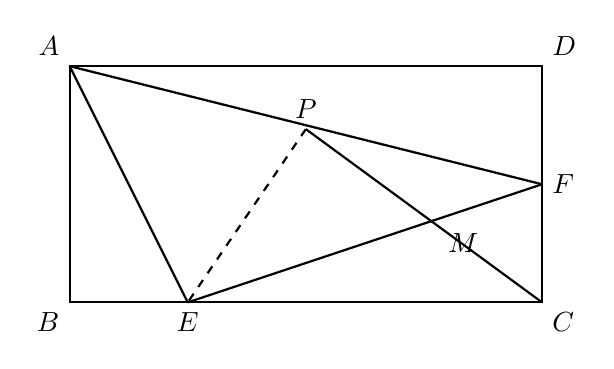
\begin{tikzpicture}[scale=0.05, line width=0.8pt]
  % Points (coordinates chosen to match the figure proportions)
  \coordinate (A) at (0,60);
  \coordinate (D) at (120,60);
  \coordinate (B) at (0,0);
  \coordinate (C) at (120,0);
  \coordinate (E) at (30,0);
  \coordinate (F) at (120,30);
  \coordinate (P) at (60,44);
  \coordinate (M) at (100,20);

  % Rectangle
  \draw (A) -- (D) -- (C) -- (B) -- cycle;

  % Edges
  \draw (A) -- (E);
  \draw (A) -- (F);
  \draw (E) -- (F);
  \draw (P) -- (C);
  \draw[dashed] (P) -- (E);

  % Labels
  \node[above left] at (A) {$A$};
  \node[above right] at (D) {$D$};
  \node[below left] at (B) {$B$};
  \node[below right] at (C) {$C$};
  \node[below] at (E) {$E$};
  \node[right] at (F) {$F$};
  \node[above] at (P) {$P$};
  \node[below] at (M) {$M$};
\end{tikzpicture}
\end{document}
